%!TEX encoding = UTF-8 Unicode
%!TEX TS-program = pdflatex

%%% --- PREAMBLE --- %%%

\documentclass[a4paper,11pt]{article}

\usepackage[italian]{babel}
\usepackage[left=2cm,right=2cm,top=2cm,bottom=2cm]{geometry}
\usepackage[T1]{fontenc} % OT1: basic, T1: western, T3 and T5: exotic, T4: lots of characters but WORSE READABILITY
\usepackage[utf8x]{inputenc} % utf8x supports more characters than utf8
\usepackage{graphicx} % import PNG, JPG and PDF with \includegraphics
\usepackage[usenames,table]{xcolor} % \color
\usepackage{amssymb}
\usepackage{amsmath}
\usepackage{amsfonts}
\usepackage{float}
\usepackage{mathtools} % (!! PLACE BEFORE hyperref !!)
\usepackage{xfrac} % \sfrac
\usepackage{cancel} % \cancel \cancelto
%\usepackage{hyperref} % interactive links in TOC, URLs and references
% unneded \usepackage{fixltx2e} % provides \textsubscript and makes some fixes
\usepackage[toc,page]{appendix}
\usepackage{siunitx} % \num \si \SI
\usepackage{alltt} % {alltt} (like verbatim but with commands)
\usepackage{moreverb} % {listing}
\usepackage{listings} % {lstlisting}
\usepackage[overload]{textcase} % fixes \MakeUppercase and \MakeLowercase
\usepackage[normalem]{ulem} % \uline \uwave \sout \xout
\usepackage{enumerate} % adds options for {enumerate}
\usepackage{paralist} % inline lists with {inparaenum}
\usepackage[official]{eurosym} % \euro
\usepackage{tabu} % {tabu} (like {tabular} with improvements)
\usepackage{layout} % layout description
\usepackage{multicol} % {multicols}
\usepackage{lipsum} % filling text generator with \lipsum
\usepackage[section]{placeins} % inhibits float figures from trepassing a section boundary
\usepackage{subfig} % \subfloat to be used inside {figure}
\usepackage{wrapfig} % {wrapfigure} (like {figure} but allows text to flow on its sides)
\usepackage{ifthen} % \ifthenelse
\usepackage{calc}
\usepackage{array}
\usepackage{multirow}
\usepackage{booktabs} % \toprule, \midrule, \bottomrule
\usepackage{fancyhdr}
\usepackage{wasysym}
\graphicspath{ {../Figs-Tabs/} } % graphics search directories
\setcounter{tocdepth}{1} % -1: part, 0: chapter, 1: section, 2: subsection, 3: subsubsection

\lstset{ %
	language=C,
	deletekeywords={},
	morekeywords={},
	backgroundcolor=\color{white},
	basicstyle=\ttfamily\small,
	commentstyle=\color{teal},
	keywordstyle=\color{magenta},
	stringstyle=\color{purple},
	identifierstyle=\color{violet!80!black},
	numbers=left,
	numbersep=7pt,
	numberstyle=\scriptsize\sffamily\color{gray},
	stepnumber=1,
	breakatwhitespace=false,
	breaklines=true,
	keepspaces=true,
	showspaces=false,
	showstringspaces=false,
	showtabs=false,
	tabsize=2,
	captionpos=none,
}

\newcommand{\ndr}[1]{\footnote{#1 (n.d.r.)}}
\newcommand{\fig}[1]{\figurename{ \ref{:#1}} %inserting reference to figures
\newcommand{\tab}[1]{\tablename{ \ref{:#1}} % inserting reference to tables
\newcommand{\eqn}[1]{equazione \eqref{eq:#1}} % inserting reference to equation
\newcommand{\dof}{\text{ dof}} % degrees of freedom
\newcommand{\paral}{\mathbin{\|}} % impedance parallel
\DeclareSIUnit\deca{decade} % decade unit definition for use in siunitx
\DeclareSIUnit\gauss{Gs} % Gauss unit definition for use in siunitx

\newcommand{\insertpart}[2]{\input{#1}}
\newcommand{\e}{\textbf{$e^{-}$}}

\sisetup{%
	separate-uncertainty = true,
	per-mode = symbol,
	bracket-numbers = false,
	multi-part-units = single,
	table-number-alignment = center,
	range-phrase = \text{--},
	range-units = single,
	output-complex-root =  \text{\ensuremath{j}},
	table-figures-decimal = 3,
	table-figures-exponent = 0,
	table-figures-integer = 2,
	table-figures-uncertainty = 2,
}

%%% --- DOCUMENT --- %%%


%%%%% SIunits example use:
% \si{\kilo\volt\per\meter\squared} -> kV/m^2
% \SI{1.222 (34)}{\joule\second}    -> 1.222 +- 0.034 Js
% \SI{1.222 \pm 0.034}{\nF}         -> 1.222 +- 0.034 nF
% use it plz

\author{Gruppo BF \\ Thomas Giannoni, Valerio Lomanto, Roberto Ribatti}
\title{Esercitazione N.11: Semplici circiti logici e mltivibratori.}
\date{9 marzo 2017}
%Intestazione
\pagestyle{fancy}
\lhead{Esperienza N.4}
\chead{Rapporto e/m}
\rhead{Gruppo BF}
\begin{document}
\maketitle
\begin{abstract}
	L'obiettivo di questa esperienza è la verifica della tabella di verità di alcni circiti logici basati s circiti integrati SN7400.
	In tale esperienza si sono realizzati ed analizzati n circito mltivibratore nonostabile, ed n circito mltivibratore astabile.


\end{abstract}

\section{Strmentazione}
In qest'esperienza esperienza sono state impiegate :
\begin{itemize}
	\item 2 circiti integrati SN7400 sati per costitire i circiti in esame
	\item varie resistenze e capacità impiegateanch'esse per il montaggio dei circiti
	\item 1 DIP switch a 4 interrttori
	\item 1 diodo 1N418
	\item 2 diodi LED, impiegati per rendere osservabile visivamente le tabelle di verità. 
	\item Il circito implsatore basato sl Ardino nano montato nell'esperienza n:10
	\item n mltimetro digitale
	\item oscilloscopio digitale 
	\item n generatore di fnzioni
\end{itemize}
\section{verifica tabella NEND}
Per la verifica della tabella di verità di na porta NEND \tablename{ \ref{t:NEND}}
\begin{table}[htb]
	\centering
	\begin{tabular}{sss}
		\toprule
		\text{ingresso} A & \text{ingresso} B &\text{scita porta NAND }$\overline{A\cdot B}$	\\
		\midrule
		0  & 0 & 1\\
		0  & 1 & 1\\
		1  & 0 & 1\\
		1  & 1 & 0\\
		\bottomrule
	\end{tabular}
	\caption{Tabella di verità di na porta NEND.}
	\label{t:NEND}
\end{table}
si è procedto in de maniere distinte; na prima verifica visiva che impiega il DIP switch in dotazione; ed na che impiega il circito implsatore basato s ardino.
Per entrambi i modi si è montato il circito in \figurename{ \ref{f:NEND}}
\begin{figure}[htb]
	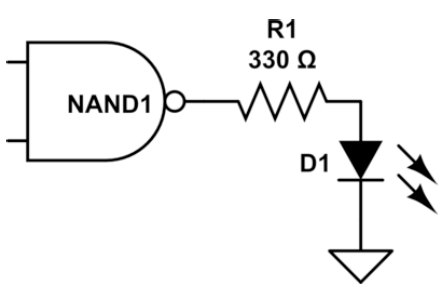
\includegraphics[scale=1.0]{NEND.png}
\end{figure}\label{f:NEND}

\section{title}

\end{document}
